\section{Addition}
\paragraph{Study1}
%To further observe the influence of uplift events for students facing stressor events,
%we statistic all the stressful intervals~\cite{Li2017Analyzing} detected surround the scheduled examinations over the 124 students during their high school career.
%For each student, we divide all his/her stressful intervals into two sets:
%1) stressful intervals under the influence of neighbouring uplift events (e.g., \emph{Halloween activity}), and 2) independent stressful intervals.
%Figure~\ref{fig:frequency} shows five measures of each student during the above two conditions:
%the \emph{accumulated stress}, the \emph{average stress} (per day), the \emph{length of stressful intervals},
%the \emph{frequency of academic topic words}, and the \emph{ratio of academic stress among all types of stress}.
%For each measure, we calculate the average value over all eligible slides for each student.
%\begin{figure}
%\centering
%\caption{Compare students' stress during exam intervals in two situations:
%1) affected by neighboring uplift events (U-SI), 2) no uplift events occurred nearby (SI)}
%\includegraphics[width=\linewidth]{figs/frequency.eps}
%\label{fig:frequency}
%\end{figure}

\paragraph{Method}
